%%%%%%%%%%%%%%%%%%%%%%%%%%%%%%%%%%%%%%%%%%%%%%%%%%%%%%%%%%%%%%%
%% OXFORD THESIS TEMPLATE

% Use this template to produce a standard thesis that meets the Oxford University requirements for DPhil submission
%
% Originally by Keith A. Gillow (gillow@maths.ox.ac.uk), 1997
% Modified by Sam Evans (sam@samuelevansresearch.org), 2007
% Modified by John McManigle (john@oxfordechoes.com), 2015
% Modified by Ulrik Lyngs (ulrik.lyngs@cs.ox.ac.uk), 2018, for use with R Markdown
%
% Ulrik Lyngs, 25 Nov 2018: Following John McManigle, broad permissions are granted to use, modify, and distribute this software
% as specified in the MIT License included in this distribution's LICENSE file.
%
% John tried to comment this file extensively, so read through it to see how to use the various options.  Remember
% that in LaTeX, any line starting with a % is NOT executed.  Several places below, you have a choice of which line to use
% out of multiple options (eg draft vs final, for PDF vs for binding, etc.)  When you pick one, add a % to the beginning of
% the lines you don't want.


%%%%% CHOOSE PAGE LAYOUT
% The most common choices should be below.  You can also do other things, like replacing "a4paper" with "letterpaper", etc.

% This one will format for two-sided binding (ie left and right pages have mirror margins; blank pages inserted where needed):
%\documentclass[a4paper,twoside]{templates/ociamthesis}
% This one will format for one-sided binding (ie left margin > right margin; no extra blank pages):
%\documentclass[a4paper]{ociamthesis}
% This one will format for PDF output (ie equal margins, no extra blank pages):
%\documentclass[a4paper,nobind]{templates/ociamthesis}
%UL 2 Dec 2018: pass this in from YAML
\documentclass[a4paper, nobind]{templates/ociamthesis}

% UL 5 January 2021 - add packages used by kableExtra
\usepackage{booktabs}
\usepackage{longtable}
\usepackage{array}
\usepackage{multirow}
\usepackage{wrapfig}
\usepackage{colortbl}
\usepackage{pdflscape}
\usepackage{tabu}
\usepackage{threeparttable}
\usepackage{threeparttablex}
\usepackage[normalem]{ulem}
\usepackage{makecell}
\usepackage[colorlinks=false,pdfpagelabels,hidelinks=true]{hyperref}
\usepackage{float}

%UL set section header spacing
\usepackage{titlesec}
% 
\titlespacing\subsubsection{0pt}{24pt plus 4pt minus 2pt}{0pt plus 2pt minus 2pt}

% UL 30 Nov 2018 pandoc puts lists in 'tightlist' command when no space between bullet points in Rmd file
\providecommand{\tightlist}{%
  \setlength{\itemsep}{0pt}\setlength{\parskip}{0pt}}
 
% UL 1 Dec 2018, fix to include code in shaded environments

%UL set whitespace around verbatim environments
\usepackage{etoolbox}
\makeatletter
\preto{\@verbatim}{\topsep=0pt \partopsep=0pt }
\makeatother

%UL 26 Mar 2019, enable strikethrough
\usepackage[normalem]{ulem}

%UL use soul package for correction highlighting
\usepackage{color, soul}
\usepackage{xcolor}
\definecolor{correctioncolor}{HTML}{CCCCFF}
\sethlcolor{correctioncolor}
\newcommand{\ctext}[3][RGB]{%
  \begingroup
  \definecolor{hlcolor}{#1}{#2}\sethlcolor{hlcolor}%
  \hl{#3}%
  \endgroup
}
\soulregister\ref7
\soulregister\cite7
\soulregister\autocite7
\soulregister\textcite7
\soulregister\pageref7

%%%%%%% PAGE HEADERS AND FOOTERS %%%%%%%%%
\usepackage{fancyhdr}
\setlength{\headheight}{15pt}
\fancyhf{} % clear the header and footers
\pagestyle{fancy}
\renewcommand{\chaptermark}[1]{\markboth{\thechapter. #1}{\thechapter. #1}}
\renewcommand{\sectionmark}[1]{\markright{\thesection. #1}} 
\renewcommand{\headrulewidth}{0pt}

\fancyhead[LO]{\emph{\leftmark}} 
\fancyhead[RE]{\emph{\rightmark}} 

% UL page number position 
\fancyfoot[C]{\emph{\thepage}} %regular pages
\fancypagestyle{plain}{\fancyhf{}\fancyfoot[C]{\emph{\thepage}}} %chapter pages

% JEM fix header on cleared pages for openright
\def\cleardoublepage{\clearpage\if@twoside \ifodd\c@page\else
   \hbox{}
   \fancyfoot[C]{}
   \newpage
   \if@twocolumn\hbox{}\newpage
   \fi
   \fancyhead[LO]{\emph{\leftmark}} 
   \fancyhead[RE]{\emph{\rightmark}} 
   \fi\fi}


%%%%% SELECT YOUR DRAFT OPTIONS
% This adds a "DRAFT" footer to every normal page.  (The first page of each chapter is not a "normal" page.)

% This highlights (in blue) corrections marked with (for words) \mccorrect{blah} or (for whole
% paragraphs) \begin{mccorrection} . . . \end{mccorrection}.  This can be useful for sending a PDF of
% your corrected thesis to your examiners for review.  Turn it off, and the blue disappears.
\correctionstrue

%%%%% BIBLIOGRAPHY SETUP
% Note that your bibliography will require some tweaking depending on your department, preferred format, etc.
% If you've not used LaTeX before, I recommend reading a little about biblatex/biber and getting started with it.
% If you're already a LaTeX pro and are used to natbib or something, modify as necessary.
% Either way, you'll have to choose and configure an appropriate bibliography format...


\usepackage[style=authoryear, sorting=nyt, backend=biber, maxcitenames=2, useprefix, doi=true, isbn=false, uniquename=false]{biblatex}
\newcommand*{\bibtitle}{Works Cited}

\addbibresource{references.bib}


% This makes the bibliography left-aligned (not 'justified') and slightly smaller font.
\renewcommand*{\bibfont}{\raggedright\small}


% Uncomment this if you want equation numbers per section (2.3.12), instead of per chapter (2.18):
%\numberwithin{equation}{subsection}


%%%%% THESIS / TITLE PAGE INFORMATION
% Everybody needs to complete the following:
\title{Methods and applications of Bayesian spatio-temporal statistics for prioritised HIV prevention}
\author{Adam Howes}
\college{Department of Mathematics}

% Master's candidates who require the alternate title page (with candidate number and word count)
% must also un-comment and complete the following three lines:

% Uncomment the following line if your degree also includes exams (eg most masters):
%\renewcommand{\submittedtext}{Submitted in partial completion of the}
% Your full degree name.  (But remember that DPhils aren't "in" anything.  They're just DPhils.)
\degree{Doctor of Philosophy}
% Term and year of submission, or date if your board requires (eg most masters)
\degreedate{September 2023}


%%%%% YOUR OWN PERSONAL MACROS
% This is a good place to dump your own LaTeX macros as they come up.

\newcommand{\Sc}{\mathcal{S}}
\newcommand{\R}{\mathcal{R}}
\newcommand{\N}{\mathcal{N}}
\newcommand{\X}{\mathcal{X}} 
\newcommand{\m}{\mathbf{m}}
\newcommand{\bu}{\mathbf{u}}
\newcommand{\bv}{\mathbf{v}}
\newcommand{\w}{\mathbf{w}}
\newcommand{\x}{\mathbf{x}}
\newcommand{\y}{\mathbf{y}}
\newcommand{\z}{\mathbf{z}}
\newcommand{\bb}{\mathbf{b}}
\newcommand{\bphi}{\bm{\phi}}
\newcommand{\brho}{\bm{\rho}}
\newcommand{\btheta}{\bm{\theta}}

\RequirePackage{bm}

% To make text superscripts shortcuts
	\renewcommand{\th}{\textsuperscript{th}} % ex: I won 4\th place
	\newcommand{\nd}{\textsuperscript{nd}}
	\renewcommand{\st}{\textsuperscript{st}}
	\newcommand{\rd}{\textsuperscript{rd}}

%%%%% THE ACTUAL DOCUMENT STARTS HERE
\begin{document}

%%%%% CHOOSE YOUR LINE SPACING HERE
% This is the official option.  Use it for your submission copy and library copy:
\setlength{\textbaselineskip}{22pt plus2pt}
% This is closer spacing (about 1.5-spaced) that you might prefer for your personal copies:
%\setlength{\textbaselineskip}{18pt plus2pt minus1pt}

% You can set the spacing here for the roman-numbered pages (acknowledgements, table of contents, etc.)
\setlength{\frontmatterbaselineskip}{17pt plus1pt minus1pt}

% UL: You can set the line and paragraph spacing here for the separate abstract page to be handed in to Examination schools
\setlength{\abstractseparatelineskip}{13pt plus1pt minus1pt}
\setlength{\abstractseparateparskip}{0pt plus 1pt}

% UL: You can set the general paragraph spacing here - I've set it to 2pt (was 0) so
% it's less claustrophobic
\setlength{\parskip}{2pt plus 1pt}

%
% Oxford University logo on title page
%
\def\crest{{
\includegraphics{templates/ic-small.pdf}}}
\renewcommand{\university}{Imperial College London}
\renewcommand{\submittedtext}{In partial fulfillment of the requirements for the degree of}


% Leave this line alone; it gets things started for the real document.
\setlength{\baselineskip}{\textbaselineskip}


%%%%% CHOOSE YOUR SECTION NUMBERING DEPTH HERE
% You have two choices.  First, how far down are sections numbered?  (Below that, they're named but
% don't get numbers.)  Second, what level of section appears in the table of contents?  These don't have
% to match: you can have numbered sections that don't show up in the ToC, or unnumbered sections that
% do.  Throughout, 0 = chapter; 1 = section; 2 = subsection; 3 = subsubsection, 4 = paragraph...

% The level that gets a number:
\setcounter{secnumdepth}{2}
% The level that shows up in the ToC:
\setcounter{tocdepth}{1}


%%%%% ABSTRACT SEPARATE
% This is used to create the separate, one-page abstract that you are required to hand into the Exam
% Schools.  You can comment it out to generate a PDF for printing or whatnot.

% JEM: Pages are roman numbered from here, though page numbers are invisible until ToC.  This is in
% keeping with most typesetting conventions.
\begin{romanpages}

% Title page is created here
\maketitle

%%%%% COPYRIGHT -- added by ATH.
\begin{copyrights}
  The copyright of this thesis rests with the author. Unless otherwise indicated, its contents are licensed under a Creative Commons Attribution-Non Commercial 4.0 International Licence (CC BY-NC).
  Under this licence, you may copy and redistribute the material in any medium or format. You may also create and distribute modified versions of the work.
  This is on the condition that: you credit the author and do not use it, or any derivative works, for a commercial purpose.
  When reusing or sharing this work, ensure you make the licence terms clear to others by naming the licence and linking to the licence text.
  Where a work has been adapted, you should indicate that the work has been changed and describe those changes.
  Please seek permission from the copyright holder for uses of this work that are not included in this licence or permitted under UK Copyright Law.
\end{copyrights}

%%%%% ORIGINALITY -- added by ATH.
\begin{originality}
  This thesis, and the work presented in it, is work that I conducted myself.
  In all cases where I describe others' work, I provide appropriate references.
\end{originality}

%%%%% DEDICATION -- If you'd like one, un-comment the following.
\begin{dedication}
  \textit{For $\sum_i u_i$ subject to side constraints}
\end{dedication}

%%%%% ACKNOWLEDGEMENTS -- Nothing to do here except comment out if you don't want it.
\begin{acknowledgements}
 	Thanks to Jeff Eaton and Seth Flaxman for supervision of this research;
 staff and students of the StatML CDT at Imperial and Oxford;
 members of the HIV Inference Group at Imperial;
 members of the Machine Learning and Global Health Network;
 the Bill \& Melinda Gates Foundation and EPSRC for funding this PhD;
 Mike McLaren, Kevin Esvelt, the Nucleic Acid Observatory team, and the Sculpting Evolution lab for hosting my visit to MIT;
 Alex Stringer for hosting my visit to Waterloo;
 the Effective Altruism community;
 my friends and family.

 \begin{flushright}
 Adam Howes \\
 Imperial College London\\
 2023
 \end{flushright}
\end{acknowledgements}

%%%%% ABSTRACT -- Nothing to do here except comment out if you don't want it.
\begin{abstract}
	Progress towards ending AIDS as a public health threat by 2030 is faltering.
Disease burden is unevenly distributed.
Effective public health response and prioritised prevention requires accurate, timely, high-resolution estimates of epidemic and demographic indicators.
Thoughtful statistical modelling is required to overcome significant data challenges.
In this thesis, I develop and apply Bayesian spatio-temporal methods for HIV surveillance.
\end{abstract}

%%%%% MINI TABLES
% This lays the groundwork for per-chapter, mini tables of contents.  Comment the following line
% (and remove \minitoc from the chapter files) if you don't want this.  Un-comment either of the
% next two lines if you want a per-chapter list of figures or tables.
  \dominitoc % include a mini table of contents

% This aligns the bottom of the text of each page.  It generally makes things look better.
\flushbottom

% This is where the whole-document ToC appears:
\tableofcontents

\listoffigures
	\mtcaddchapter
  	% \mtcaddchapter is needed when adding a non-chapter (but chapter-like) entity to avoid confusing minitoc

% Uncomment to generate a list of tables:
\listoftables
  \mtcaddchapter
%%%%% LIST OF ABBREVIATIONS
% This example includes a list of abbreviations.  Look at text/abbreviations.tex to see how that file is
% formatted.  The template can handle any kind of list though, so this might be a good place for a
% glossary, etc.
%tibble(
%  Term = c("HIV"),
%  Abbreviation = C("Human Immunodeficiency Virus")
%  ) %>%
%  arrange(Term) %>%
%  kable(booktab = TRUE, escape = FALSE, "latex")

% After writing, reorder these as they appear in the text

% First parameter can be changed eg to "Glossary" or something.
% Second parameter is the max length of bold terms.
\begin{mclistof}{List of Abbreviations}{3.2cm}

\item[HIV] Human Immunodeficiency Virus.
\item[DALY] Disability Adjusted Life Year.
\item[AIDS] Acquired ImmunoDeficiency Syndrome.
\item[UNAIDS] The Joint United Nations Programme on HIV/AIDS.
\item[PEPFAR] President’s Emergency Plan for AIDS Relief.
\item[Global Fund] Global Fund to Fight AIDS, Tuberculosis, and Malaria.
\item[HIV] Demographic and Health Surveys.
\item[AIS] AIDS Indicator Survey.
\item[PrEP] Pre-Exposure Prophylaxis.
\item[PEP] Post-Exposure Prophylaxis.
\item[FSW] Female Sex Worker(s).
\item[MSM] Men who have Sex with Men.
\item[PWID] People Who Inject Drugs.
\item[TGP] Transgender People
\item[ANC] Antenatal Clinic.
\item[CDC] Centers for Disease Control and Prevention.
\item[UAT] Unlinked Anonymous Testing.
\item[PMTCT] Prevention of Mother-to-Child Transmission.
\item[PLHIV] People Living with HIV.
\item[TaSP] Treatment as Prevention.
\item[STI] Sexually Transmitted Infection.
\item[ART] Antiretroviral Therapy.
\item[VMMC] Voluntary Medical Male Circumcision.
\item[DHS] Demographic and Health Surveys.
\item[PHIA] Population-based HIV Impact Assessment.
\item[SSA] Sub-Saharan Africa.

\item[DDC] Data Defect Correlation.
\item[MCMC] Markov Chain Monte Carlo.
\item[NUTS] No-U-Turn Sampler.
\item[VI] Variational Inference.
\item[INLA] Integrated Nested Laplace Approximation.
\item[GP] Gaussian Process.
\item[CAR] Conditionally Auto-regressive.
\item[ICAR] Intrinsic Conditionally Auto-regressive.
\item[SAE] Small-Area Estimation.
\item[GMRF] Gaussian Markov Random Field.
\item[HMC] Hamiltonian Monte Carlo.
\item[GMRF] Gauss-Markov Random Field.
\item[HMC] Hamiltonian Monte Carlo.
\item[LM] Linear Model.
\item[GLM] Generalised Linear Model.
\item[GLMM] Generalised Linear Mixed effects Model.
\item[LGM] Latent Gaussian Model.
\item[ELGM] Extended Latent Gaussian Model.
\item[BF] Bayes Factor.
\item[CPO] Conditional Predictive Ordinate.
\item[DIC] Deviance Information Criterion.
\item[BIC] Bayesian Information Criterion.
\item[WAIC] Watanabe-Akaike Information Criterion.
\item[SR] Scoring Rule.
\item[SPSR] Strictly Proper Scoring Rule.
\item[CRPS] Continuous Ranked Probability Score.
\item[LS] Log Score.
\item[PIT] Probability Integral Transform.
\item[ECDF] Empirical Cumulative Difference Function.
\item[ESS] Effective Sample Size.
\item[IID] Independent and Identically Distributed.
\item[PPL] Probabilistic Programming Language.
\item[CCD] Central Composite Design.
\item[EB] Empirical Bayes.
\item[AGHQ] Adaptive Gauss-Hermite Quadrature.

\end{mclistof} 


%%%%% LIST OF NOTATION
\begin{mclistof}{List of Notations}{3.2cm}

\item[$\rho$] HIV prevalence.
\item[$\lambda$] HIV incidence.
\item[$\alpha$] ART coverage.
\item[$\mathcal{S}$] Spatial study region $\mathcal{S} \subseteq \mathbb{R}^2$.
\item[$s \in \mathcal{S}$] Point location.
\item[$\mathcal{T}$] Temporal study period $\mathcal{T} \subseteq \mathbb{R}$.
\item[$t \in \mathcal{T}$] Time.
\item[$\y$] Data, a $n$-vector.
\item[$\bphi$] Parameters, a $d$-vector $(\phi_1, \ldots, \phi_d)$.
\item[$\x$] Latent field, a $N$-vector $(x_1, \ldots, x_N)$.
\item[$\btheta$] Hyperparameters, a $m$-vector $(\theta_1, \ldots, \theta_m)$.
\item[$x \sim p(x)$] $x$ is distributed according to $p(x)$.
\item[$A_i$] Areal unit.
\item[$A_i \sim A_j$] Adjacency between areal units.
\item[$\mathbf{H}$] Hessian matrix.
\item[$\mathbf{R}$] Structure matrix.
\item[$\mathbf{Q}$] Precision matrix.
\item[$\bm{\Sigma}$] Covariance matrix.
\item[$\mathcal{N}$] Gaussian distribution.
\item[$k: \mathcal{X} \times \mathcal{X} \to \mathbb{R}$] Kernel function on the space $\mathcal{X}$.
\item[$A_i \sim A_j$] Adjacency between areal units.
\item[$\mathcal{Q}$] A set of quadrature nodes.
\item[$\omega: \mathcal{Q} \to \mathbb{R}$] A quadrature weighting function.
\item[$\mathcal{Q}(m, k)$] Gauss-Hermite quadrature points in $m$ dimensions with $k$ nodes per dimension, constructed according to a product rule.

\end{mclistof} 

% The Roman pages, like the Roman Empire, must come to its inevitable close.
\end{romanpages}

%%%%% CHAPTERS
% Add or remove any chapters you'd like here, by file name (excluding '.tex'):
\flushbottom

% all your chapters and appendices will appear here
\hypertarget{introduction}{%
\chapter{Introduction}\label{introduction}}

\adjustmtc
\markboth{Introduction}{}

This thesis is about applied and methodological Bayesian statistics.
The focus is on questions motivated by surveillance of HIV in sub-Saharan Africa.
The data are related to people, located in space and time.
Tackling substantive applied questions has been a productive strategy for the statistical science discipline.
As such, it is my hope that the work contained within will also be of interest more broadly.

\hypertarget{chapter-overview}{%
\section{Chapter overview}\label{chapter-overview}}

\begin{itemize}
\tightlist
\item
  Chapter \ref{background}: I review the required background for the rest of the thesis.
\item
  Chapter \ref{beyond-borders}: I raise concerns with the prevailing model for spatial structure used in small-area estimation, and evaluate whether these concerns have practical consequences \autocite{howes2023beyond}.
\item
  Chapter \ref{multi-agyw}: I estimate the size of HIV risk groups for adolescent girls and young women across 13 countries in sub-Saharan Africa \autocite{howes2023spatio}.
\item
  Chapter \ref{naomi-aghq}: I develop an approximate Bayesian inference method combining adaptive Gauss-Hermite quadrature with principal components analysis, and apply it to the Naomi small-area estimation model in Malawi \autocite{howes2023fast}.
\item
  Chapter \ref{conclusions}: I discuss avenues for future work, and my conclusions regarding the PhD research.
\end{itemize}

\hypertarget{background}{%
\chapter{Background}\label{background}}

\adjustmtc
\markboth{Background}{}

\hypertarget{the-hivaids-epidemic}{%
\section{The HIV/AIDS epidemic}\label{the-hivaids-epidemic}}

According to latest estimates, in 2022 there were thirty-eight million people living with HIV, seven hundred thousand AIDS-related deaths, and one million, seven hundred thousand people newly infected with HIV.

Disease burden is unevenly distributed in space, and across communities and individuals.
The region most affected is Sub-Saharan Africa.
Key populations include men who have sex with men, female sex workers, people who inject drugs, transgender people, incarcerated people.
Large demographic groups at higher risk include adolescent girls and young women.
Fortunately, progress is being made.

Key interventions are ART, condoms, PrEP and PEP, education, economic empowerment, VMMC.

Methods for prevention prioritisation include geographic, demographic, key population services, risk screening, individual-level risk characteristics.
Are there differences in effectiveness of treatments for different groups.

Surveillance is used is conducted to track epidemic trends, identify at-risk populations, find drivers of transmission, and evaluate the impact of prevention and treatment programs.
Key HIV indicators are HIV prevalence, HIV incidence, coverage of ART and other interventions.

There are significant data related difficulties associated with furnishing these estimates.
These include sparsity in space and time, survey bias, conflicting information sources, hard to reach populations, changing demographies.
These data limitations foreground the importance of synthesising multiple sources of information to obtain estimates.
Doing so increases the difficulty and complexity of the statistical modelling required.

Aims for HIV response going forward, and surveillance capabilities are needed to meet them.
Phasing out of nationally-representative household surveys for HIV.

\hypertarget{bayesian-spatio-temporal-statistics}{%
\section{Bayesian spatio-temporal statistics}\label{bayesian-spatio-temporal-statistics}}

\hypertarget{bayesian-statistics}{%
\subsection{Bayesian statistics}\label{bayesian-statistics}}

Bayesian statistics is a paradigm for learning from data.
In this section I will provide a brief overview.
For a more complete introduction, I recommend \textcite{mcelreath2020statistical} or \textcite{gelman2013bayesian}.

At it's best, the Bayesian framework allows the analyst focus their attention on modelling the data at hand.
In particular, this is achieved by the construction of a generative model for the observed data \(y\) together with parameters \(\vartheta\)
\begin{equation}
(y, \vartheta) \sim p(y, \vartheta).
\end{equation}
Given this generative model, computation of the posterior distribution
\begin{equation}
p(\vartheta \, | \, y) = \frac{p(y \, | \, \vartheta) p(\vartheta)}{p(y)}, \label{eq:posterior}
\end{equation}
usually proceeds using approximate Bayesian inference methods, where \(p(y \, | \, \vartheta)\) is the likelihood, \(p(y \, | \, \vartheta)\) is the prior, and \(p(\vartheta)\) is the evidence.

Markov chain Monte Carlo (MCMC) is the most popular approach for computing Equation \ref{eq:posterior}, and proceeds by simulating samples from a Markov chain with stationary distribution equal to the distribution of interest.
Variational Bayes approaches assume the posterior distribution belongs to some class and use optimisation to choose the best member of that class.
Particular properties of spatio-temporal models make integrated nested Laplace approximations, if feasible, often the best option
Empirical Bayes approaches, like Template Model Builder \autocite{osgoodzimmerman2021statistical}.

\hypertarget{spatio-temporal-statistics}{%
\subsection{Spatio-temporal statistics}\label{spatio-temporal-statistics}}

In spatio-temporal statistics the data we observe are indexed by spatial or temporal location.
Commonly used independent and identically distributed (IID) assumptions on observations are rarely suitable in this setting because we expect there to be spatio-temporal correlation structure.

Split the parameters \(\vartheta = (x, \theta)\).
Call \(x\) the latent field.
Call \(\theta\) the hyperparameters.
Often, the latent field is assumed to be jointly multivariate Gaussian.

\hypertarget{latent-gaussian-and-extended-latent-gaussian-models}{%
\subsection{Latent Gaussian and extended latent Gaussian models}\label{latent-gaussian-and-extended-latent-gaussian-models}}

Latent Gaussian models \autocite{rue2009approximate} are of the form
\begin{align*}
y_i &\sim p(y_i \, | \, \eta_i, \theta_1), \quad i \in [n]\\
\mu_i &= \mathbb{E}(y_i \, | \, \eta_i) = g(\eta_i), \\
\eta_i &= \beta_0 + \sum_{l = 1}^{p} \beta_j z_{ji} + \sum_{k = 1}^{r} f_k(u_{ki}),
\end{align*}
where \([n] = \{1, \ldots, n\}\).
The response variable is \(y = (y)_{i \in [n]}\) with likelihood \(p(y \, | \, \eta, \theta_1) = \prod_{i = 1}^n p(y_i \, | \, \eta_i, \theta_1)\), where \(\eta = (\eta)_{i \in [n]}\).
Each response has conditional mean \(\mu_i\) with inverse link function \(g: \mathbb{R} \to \mathbb{R}\) such that \(\mu_i = g(\eta_i)\).
The vector \(\theta_1 \in \mathbb{R}^s\), with \(s_1\) assumed small, are additional parameters of the likelihood.
The structured additive predictor \(\eta_i\) may include an intercept \(\beta_0\), linear effects \(\beta_j\) of the covariates \(z_{ji}\), and unknown functions \(f_k(\cdot)\) of the covariates \(u_{ki}\).
The parameters \(\beta_0\), \(\{\beta_j\}\), \(\{f_k(\cdot)\}\) are each assigned Gaussian priors.
It is convenient to collect these parameters into a vector \(x \in \mathbb{R}^N\) called the latent field such that \(x \sim \mathcal{N}(0, Q(\theta_2)^{-1})\) where \(\theta_2 \in \mathbb{R}^{s_2}\) are further parameters, again with \(s_2\) assumed small.
Let \(\theta = (\theta_1, \theta_2) \in \mathbb{R}^s\) with \(m = s_1 + s_2\) be all hyperparameters, with prior \(p(\theta)\).
Common examples of latent Gaussian models include the following.

Many of the leading-edge models used in small-area estimation fall outside the latent Gaussian model class.
Examples include disaggregation models, evidence synthesis models \autocite{eaton2019joint,eaton2021naomi}, attendance models, risk group models.
However, many of these models do fit into the class of extended latent Gaussian models \autocite{stringer2021fast}.
By allowing many-to-one link functions, extended latent Gaussian models facilitate modelling of non-linearities.

\hypertarget{survey-methods}{%
\subsection{Survey methods}\label{survey-methods}}

\hypertarget{beyond-borders}{%
\chapter{Spatial structure}\label{beyond-borders}}

\adjustmtc
\markboth{Models for spatial structure}{}

Code for the analysis in this chapter is available from \href{https://github.com/athowes/beyond-borders}{\texttt{athowes/beyond-borders}} and supported by the R package \href{https://athowes.github.io/arealutils}{\texttt{arealutils}}.
Include an edited version of the corresponding paper here.

\hypertarget{background-1}{%
\section{Background}\label{background-1}}

\hypertarget{areal-and-point-data}{%
\subsection{Areal and point data}\label{areal-and-point-data}}

\hypertarget{spatial-random-effects}{%
\subsection{Spatial random effects}\label{spatial-random-effects}}

\hypertarget{models-based-on-adjacency}{%
\section{Models based on adjacency}\label{models-based-on-adjacency}}

\hypertarget{the-besag-model}{%
\subsection{The Besag model}\label{the-besag-model}}

\hypertarget{the-bym2-model}{%
\subsection{The BYM2 model}\label{the-bym2-model}}

\hypertarget{models-using-kernels}{%
\section{Models using kernels}\label{models-using-kernels}}

\hypertarget{the-centroid-kernel-model}{%
\subsection{The centroid kernel model}\label{the-centroid-kernel-model}}

\hypertarget{the-integrated-kernel-model}{%
\subsection{The integrated kernel model}\label{the-integrated-kernel-model}}

\hypertarget{simulation-study}{%
\section{Simulation study}\label{simulation-study}}

\hypertarget{synthetic-data-sets}{%
\subsection{Synthetic data-sets}\label{synthetic-data-sets}}

\hypertarget{inferential-models}{%
\subsection{Inferential models}\label{inferential-models}}

\hypertarget{priors}{%
\subsubsection{Priors}\label{priors}}

\hypertarget{kernel-details}{%
\subsubsection{Kernel details}\label{kernel-details}}

\hypertarget{inference-algorithms}{%
\subsection{Inference algorithms}\label{inference-algorithms}}

\hypertarget{model-assessment}{%
\subsection{Model assessment}\label{model-assessment}}

\hypertarget{continuous-ranked-probability-score}{%
\subsubsection{Continuous ranked probability score}\label{continuous-ranked-probability-score}}

\hypertarget{results}{%
\subsection{Results}\label{results}}

\hypertarget{hiv-prevalence-study}{%
\section{HIV prevalence study}\label{hiv-prevalence-study}}

\hypertarget{results-1}{%
\subsection{Results}\label{results-1}}

\hypertarget{discussion}{%
\section{Discussion}\label{discussion}}

\hypertarget{limitations}{%
\subsection{Limitations}\label{limitations}}

\hypertarget{conclusion}{%
\subsection{Conclusion}\label{conclusion}}

\hypertarget{multi-agyw}{%
\chapter{A model for risk group proportions}\label{multi-agyw}}

\adjustmtc
\markboth{A model for risk group proportions}{}

In this chapter I describe an application of Bayesian spatio-temporal statistics to small-area estimation of HIV risk group proportions.
This work was done in collaboration with colleagues from the MRC Centre for Global Infectious Disease Analysis and UNAIDS.
My primary role was to develop the statistical model, building upon an earlier version of the analysis conducted by Kathryn Risher.
The results are described in \textcite{howes2023spatio}, and are beginning to be used by countries to guide policy via a spreadsheet tool created by Kathryn.
Code for the analysis in this chapter is available from \href{https://github.com/athowes/multi-agyw}{\texttt{athowes/multi-agyw}} and supported by the R package \href{https://athowes.github.io/multi.utils}{\texttt{multi.utils}}.

\hypertarget{background-2}{%
\section{Background}\label{background-2}}

Risk of acquiring HIV infection is not equal for all individuals.
Moreover, variation in risk is systematic across to demographic characteristics.
Adolescent girls and young women (AGYW) -- that is, females aged 15-29 -- are one demographic group at particular risk.

The Global AIDS Strategy 2021-2026 proposed stratifying HIV prevention packages to AGYW based on local population-level HIV incidence and individual-level sexual risk behaviour.
The idea is that prioritisation based on both of these factors is more efficient than on only or one the other.

\begin{figure}

{\centering 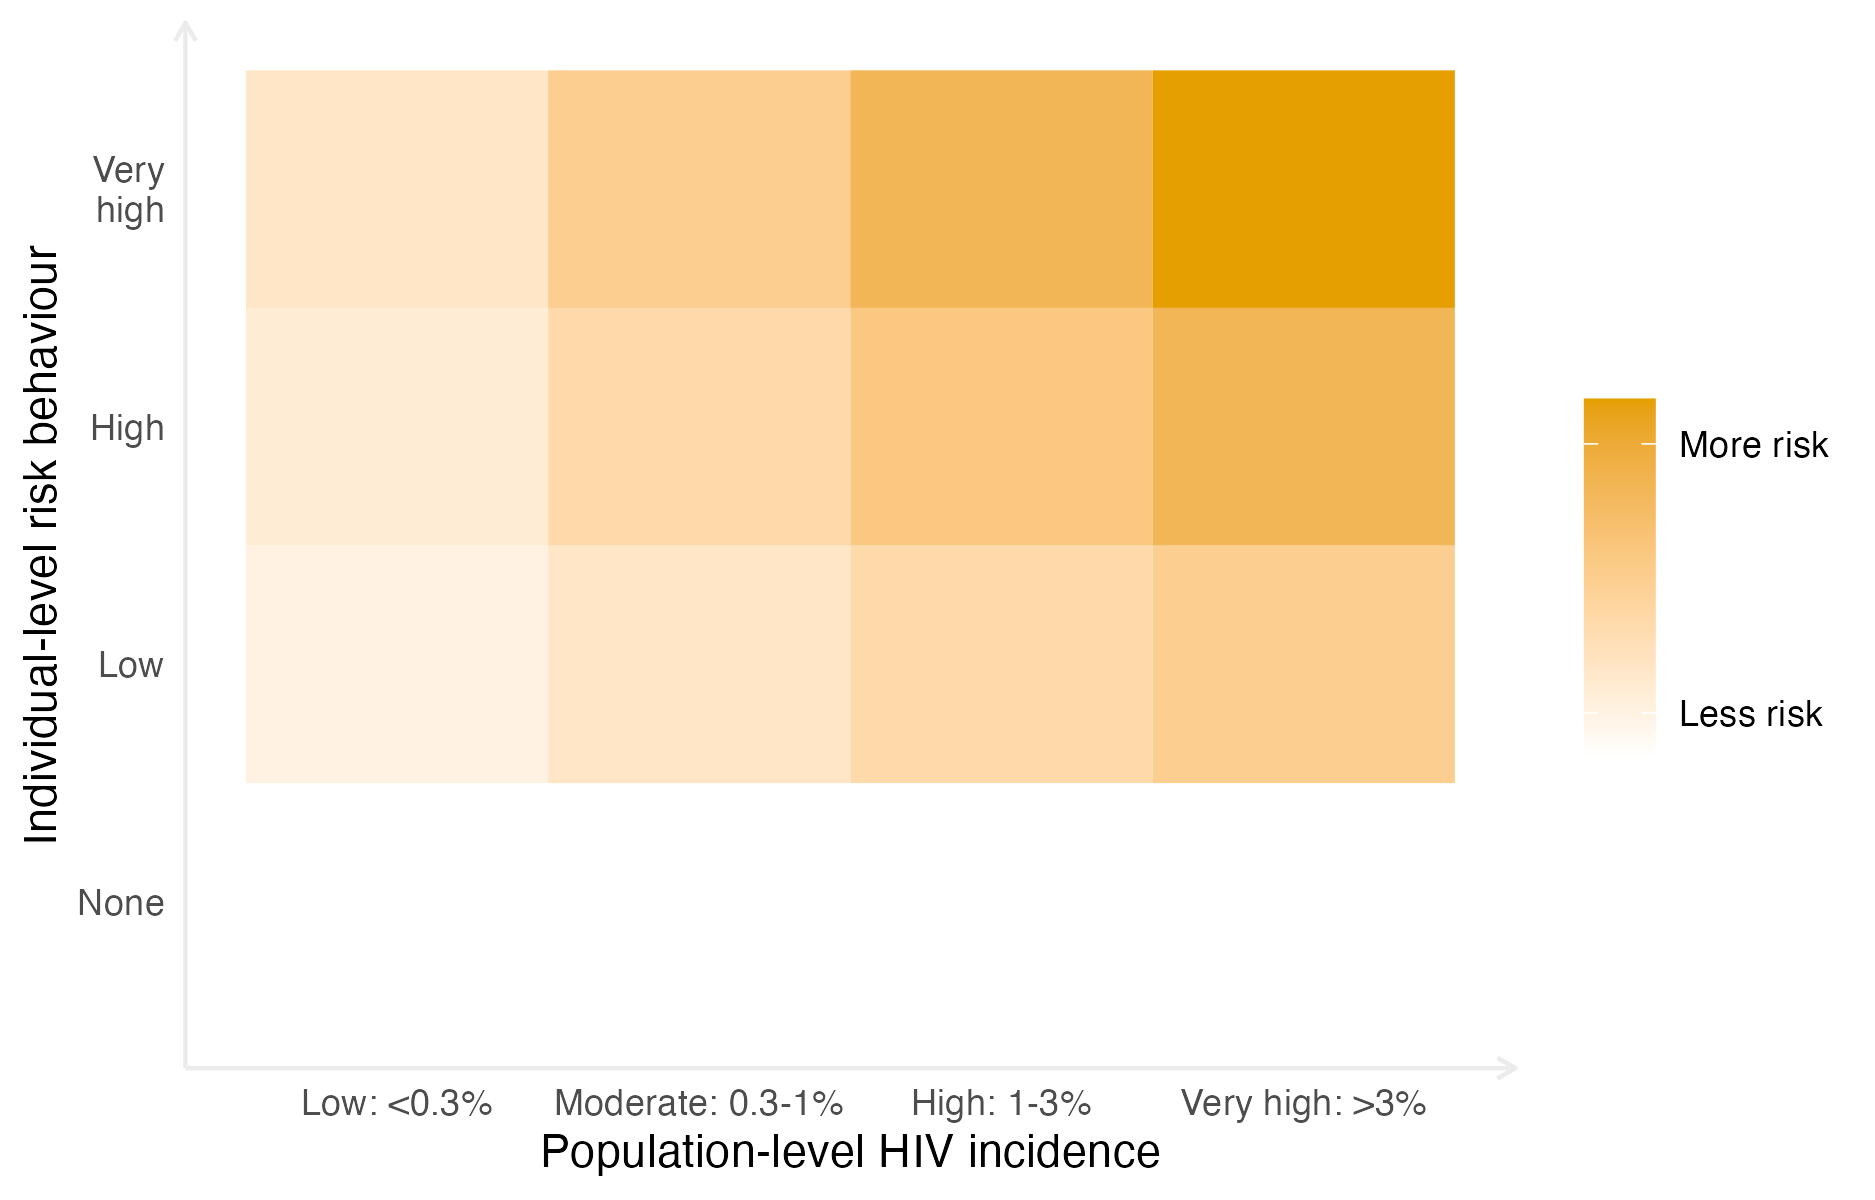
\includegraphics[width=0.9\linewidth]{figures/extra/risk-grid} 

}

\caption{Risk grid.}\label{fig:risk-grid}
\end{figure}

Implementing the strategy requires estimates.

\hypertarget{data}{%
\section{Data}\label{data}}

I used household survey data.

\hypertarget{model-for-risk-group-proportions}{%
\section{Model for risk group proportions}\label{model-for-risk-group-proportions}}

I found that it was not appropriate to use the surveys without a specific transactional sex question on an equal footing to the other surveys.
For this reason, I took a two-stage modelling approach to estimate the four risk group proportions.
In particular, index the four risk groups as \(k \in \{1, 2, 3, 4\}\), and denote being in either the third or fourth risk group by \(k = 3^{+}\).
First, using all the surveys, I used a multinomial logistic regression model to model the proportion of AGYW in the risk groups \(k \in \{1, 2, 3^{+}\}\).
Then, using only those surveys with a specific transactional sex question, I fit a logistic regression model to estimate the proportion of those in the \(k = 3^{+}\) risk group that were in the \(k = 3\) and \(k = 4\) risk groups respectively.

\hypertarget{spatio-temporal-multinomial-logistic-regression}{%
\subsection{Spatio-temporal multinomial logistic regression}\label{spatio-temporal-multinomial-logistic-regression}}

Let \(i \in \{1, \ldots, n\}\) denote districts which partition the 13 studied AGYW priority countries \(c[i] \in \{1, \ldots, 13\}\).
Consider the years 1999-2018 denoted as \(t \in \{1, \ldots, T\}\), and age groups \(a \in \{\text{15--19}, \text{20--24}, \text{25--29}\}\).
Let \(p_{itak} > 0\) with \(\sum_{k = 1}^{3^{+}} p_{itak} = 1\), be the probability of membership of risk group \(k\) for an individual in district \(i\), at time \(t\), in age group \(a\).

\hypertarget{multinomial-logistic-regression}{%
\subsubsection{Multinomial logistic regression}\label{multinomial-logistic-regression}}

A baseline category multinomial logistic regression model is specified by
\begin{align}
    \y_{ita} &= (y_{ita1}, \ldots, y_{ita3^{+}})^\top \sim \text{Multinomial}(m_{ita}; \, p_{ita1}, \ldots, p_{ita3^{+}}), \\
    \log(p_{itak} / p_{ita1}) &= \eta_k, k = 2, 3^{+},
\end{align}
where the number in risk group \(k\) is \(y_{itak}\), the sample size is \(m_{ita} = \sum_{k = 1}^{3^{+}} y_{itak}\), \(p_{itak} > 0\) is the probability of membership of the \(k\)th risk group, and \(k = 1\) is the baseline category.

\hypertarget{the-multinomial-poisson-transformation}{%
\subsubsection{The multinomial-Poisson transformation}\label{the-multinomial-poisson-transformation}}

The multinomial-Poisson transformation reframes a given multinomial logisitic regression model as an equivalent Poisson log-linear model of the form
\begin{align}
    y_{itak} &\sim \text{Poisson}(\kappa_{itak}), \label{eq:poisson} \\
    \log(\kappa_{itak}) &= \eta_{itak},
\end{align}
for certain choice of the linear predictor \(\eta_{itak}\).
The basis of the transformation is that, conditional on their sum, Poisson counts are jointly multinomially distributed \autocite{mccullagh1989generalized} as follows
\begin{equation}
    \mathbf{y}_{ita} \, | \, m_{ita} \sim \text{Multinomial} \left( m_{ita}; \frac{\kappa_{ita1}}{\kappa_{ita}}, \ldots, \frac{\kappa_{ita3^{+}}}{\kappa_{ita}} \right),
\end{equation}
where \(\kappa_{ita} = \sum_{k = 1}^{3^{+}} \kappa_{itak}\) such that category probabilities are obtained by the softmax function
\begin{equation}
    p_{itak} = \frac{\exp(\eta_{itak})}{\sum_{k = 1}^{3^{+}} \exp(\eta_{itak})} = \frac{\kappa_{itak}}{\sum_{k = 1}^{3^{+}} \kappa_{itak}} = \frac{\kappa_{itak}}{\kappa_{ita}}.
\end{equation}
In the equivalent model, the sample sizes \(m_{ita} = \sum_k y_{itak}\) are treated as random, rather than fixed as they would be in the multinomial logistic regression model, taking a Poisson distribution
\begin{equation}
    m_{ita} \sim \text{Poisson} \left( \kappa_{ita} \right).
\end{equation}
In the equivalent model, the joint distribution of \(p(\mathbf{y}_{ita}, m_{ita}) = p(\mathbf{y}_{ita} \, | \, m_{ita})p(m_{ita})\) is
\begin{align}
p(\mathbf{y}_{ita}, m_{ita}) &= \exp(-\kappa_{ita}) \frac{(\kappa_{ita})^{m_{ita}}}{m_{ita}!} \times \frac{m_{ita}!}{\prod_k y_{itak}!} \prod_k \left( \frac{\kappa_{itak}}{\kappa_{ita}} \right)^{y_{itak}} \\
&= \prod_k \left( \frac{\exp(-\kappa_{itak}) \left( \kappa_{itak} \right)^{y_{itak}}}{y_{itak}!} \right) \\
&= \prod_k \text{Poisson} \left( y_{itak} \, | \, \kappa_{itak} \right). \label{eq:prodpoisson}
\end{align}
corresponding to the product of independent Poisson likelihoods as in Equation \ref{eq:poisson}.
This model, including random sample sizes, is equivalent to the multinomial logistic regression only when these normalisation constants are recovered exactly.
To ensure that this is the case, one approach is to include observation-specific random effects \(\theta_{ita}\) in the equation for the linear predictor.
Multiplying each of \(\{\kappa_{itak}\}_{k = 1}^{3^+}\) by \(\exp(\theta_{ita})\) has no effect on the category probabilities, but does provide the necessary flexibility for \(\kappa_{ita}\) to recover \(m_{ita}\) exactly.
Although in theory an improper prior \(\theta_{ita} \propto 1\) should be used, in practise, by keeping \(\eta_{ita}\) otherwise small using appropriate constraints, so that arbitrarily large values of \(\theta_{ita}\) are not required, it is sufficient (and practically preferable for inference) to instead use a vague prior.

\hypertarget{model-specifications}{%
\subsubsection{Model specifications}\label{model-specifications}}

I considered four models for \(\eta_{ita}\) of the form
\[
\eta_{ita} = \theta_{ita} + \beta_k + \zeta_{c[i]k} + \alpha_{ac[i]k} + \phi_{ik} + \gamma_{tk}.
\]
Observation random effects \(\theta_{ita} \sim \mathcal{N}(0, 1000^2)\) were included in all models we considered.
To capture country-specific proportion estimates for each category, we included category random effects \(\beta_k \sim \mathcal{N}(0, \tau_\beta^{-1})\) and country-category random effects \(\zeta_{ck} \sim \mathcal{N}(0, \tau_\zeta^{-1})\).
Heterogeneity in risk group proportions by age was allowed by including age-country-category random effects \(\alpha_{ack} \sim \mathcal{N}(0, \tau_\alpha^{-1})\).
I considered two specifications, independent and identically distributed (IID) and Besag \autocite{besag1991bayesian}, for the space-category \(\phi_{ik}\) random effects (Section \ref{sec:spatial-random-effects}) and two specifications, IID and first order autoregressive (AR1), for the year-category \(\gamma_{tk}\) random effects (Section \ref{sec:temporal-random-effects}).
All random effect precision parameters \(\tau \in \{\tau_\beta, \tau_\zeta, \tau_\alpha, \tau_\phi, \tau_\gamma\}\) were given independent penalised complexity (PC) priors \autocite{simpson2017penalising} with base model \(\sigma = 0\) given by \(p(\tau) = 0.5 \nu \tau^{-3/2} \exp \left( - \nu \tau^{-1/2} \right)\) where \(\nu = - \ln(0.01) / 2.5\) such that \(\mathbb{P}(\sigma > 2.5) = 0.01\).

\hypertarget{spatial-random-effects-1}{%
\subsubsection{Spatial random effects}\label{spatial-random-effects-1}}

The specifications we considered were IID
\[
\phi_{ik} \sim \mathcal{N}(0, \tau_\phi^{-1}),
\]
and Besag grouped by category
\[
\bphi = (\phi_{11}, \ldots, \phi_{n1}, \ldots, \phi_{1{3^{+}}}, \ldots \phi_{n3^{+}})^\top \sim \mathcal{N}(\mathbf{0}, (\tau_\phi \mathbf{R}^\star_\phi)^{-}),
\]
where the scaled structure matrix \(\mathbf{R}^\star_\phi = \mathbf{R}^\star_b \otimes \mathbf{I}\) is given by the Kronecker product of the scaled Besag structure matrix \(\mathbf{R}^\star_b\) and the identity matrix \(\mathbf{I}\), and \({-}\) denotes the generalised matrix inverse.
Scaling of the structure matrix to have generalised variance one ensures interpretable priors may be placed on the precision parameter \autocite{sorbye2014scaling}.
We followed the further recommendations of \textcite{freni2018note} with regard to disconnected adjacency graphs, singletons and constraints.
The Besag structure matrix \(\mathbf{R}_b\) is obtained by the precision matrix of the random effects \(\mathbf{b} = (b_1, \ldots, b_n)^\top\) with full conditionals
\begin{equation}
b_i \, | \, \mathbf{b}_{-i} \sim \N\left(\frac{\sum_{j: j \sim i} b_j}{n_{\delta i}}, \frac{1}{n_{\delta i}}\right),
\end{equation}
where \(j \sim i\) if the districts \(A_i\) and \(A_j\) are adjacent, and \(n_{\delta i}\) is the number of districts adjacent to \(A_i\).

In preliminary testing, we excluded spatial random effects from the model, but found that this negatively effected performance.
We also tested using the BYM2 model \autocite{simpson2017penalising} in place of the Besag, but found that the proportion parameter posteriors tended to be highly peaked at the value one.
For simplicity and to avoid numerical issues, by using Besag random effects we decided to fix this proportion to one.

\hypertarget{temporal-random-effects}{%
\subsubsection{Temporal random effects}\label{temporal-random-effects}}

The specifications we considered were IID
\[
\phi_{tk} \sim \mathcal{N}(0, \tau_\phi^{-1}),
\]
and AR1 grouped by category
\[
\bm{\gamma} = (\gamma_{11}, \ldots, \gamma_{13^{+}}, \ldots, \gamma_{T1}, \ldots, \gamma_{T3^{+}})^\top \sim \mathcal{N}(\mathbf{0}, (\tau_\phi \mathbf{R}^\star_\gamma)^{-}),
\]
where the scaled structure matrix \(\mathbf{R}^\star_\gamma = \mathbf{R}^\star_r \otimes \mathbf{I}\) is given by the Kronecker product of a scaled AR1 structure matrix \(\mathbf{R}^\star_r\) and the identity matrix \(\mathbf{I}\).
The AR1 structure matrix \(\mathbf{R}_r\) is obtained by precision matrix of the random effects \(\mathbf{r} = (r_1, \ldots, r_T)^\top\) specified by
\begin{align}
r_1 &\sim \left( 0, \frac{1}{1 - \rho^2} \right), \\
r_t &= \rho r_{t - 1} + \epsilon_t, \quad t = 2, \ldots, T, 
\end{align}
where \(\epsilon_t \sim \mathcal{N}(0, 1)\) and \(|\rho| < 1\).
For the lag-one correlation parameter \(\rho\), we used the PC prior, as derived by \textcite{sorbye2017penalised}, with base model \(\rho = 1\) and condition \(\mathbb{P}(\rho > 0 = 0.75)\).
We chose the base model \(\rho = 1\) corresponding to no change in behaviour over time, rather than the alternative \(\rho = 0\) corresponding to no correlation in behaviour over time, as we judged the former to be more plausible a priori.

\hypertarget{constraints}{%
\subsubsection{Constraints}\label{constraints}}

To ensure interpretable posterior inferences of random effect contribution, we applied sum-to-zero constraints such that none of the category interaction random effects altered overall category probabilities.
For the space-year-category random effects, we applied analogous sum-to-zero constraints to maintain roles of the space-category and year-category random effects.
Together, these were:

\begin{enumerate}
\def\labelenumi{\arabic{enumi}.}
\tightlist
\item
  Category \(\sum_k \beta_k = 0\)
\item
  Country \(\sum_c \zeta_{ck} = 0, \, \forall \, k\)
\item
  Age-country \(\sum_a \alpha_{ack} = 0, \, \forall \, c, k\),
\item
  Spatial \(\sum_i \phi_{ik} = 0, \, \forall \, k\)
\item
  Temporal \(\sum_t \gamma_{tk} = 0, \, \forall \, k\)
\end{enumerate}

\hypertarget{survey-weighted-likelihood}{%
\subsubsection{Survey weighted likelihood}\label{survey-weighted-likelihood}}

We included surveys which use a complex design, in which each individual has an unequal probability of being included in the sample.
For example the DHS often employs a two-stage cluster design, first taking an urban rural stratified sample of ennumeration areas, before selecting households from each ennumeration area using systematic sampling \autocite{measure2012sampling}.

To account for this aspect of survey design, we use a weighted pseudo-likelihood where the observed counts \(y\) are replaced by effective counts \(y^\star\) calculated using the survey weights \(w_j\) of all individuals \(j\) in the corresponding strata.
We multiplied direct estimates produced using the \texttt{survey} package \autocite{JSSv009i08} by the Kish effective sample size \autocite{kish1965survey}
\begin{equation}
    m^\star = \frac{\left(\sum_j w_j \right)^2}{\sum_j {w_j}^2}
\end{equation}
to obtain \(y^\star\).
These counts may not be integers, and as such the Poisson likelihood we used in Equation \ref{eq:poisson} is not appropriate.
Instead, we used a generalised Poisson pseudo-likelihood \(y^\star \sim \text{xPoisson}(\kappa)\), given by
\begin{equation}
    p(y^\star) = \frac{\kappa^{y^\star}}{\left \lfloor{y^\star!}\right \rfloor } \exp \left(- \kappa \right),
\end{equation}
as implemented by \texttt{family\ =\ "xPoisson"} in \texttt{R-INLA}, which accepts non-integer input.

\hypertarget{model-selection}{%
\subsubsection{Model selection}\label{model-selection}}

\hypertarget{spatial-logistic-regression}{%
\subsection{Spatial logistic regression}\label{spatial-logistic-regression}}

\hypertarget{model-specifications-1}{%
\subsubsection{Model specifications}\label{model-specifications-1}}

\hypertarget{survey-weighted-likelihood-1}{%
\subsubsection{Survey weighted likelihood}\label{survey-weighted-likelihood-1}}

\hypertarget{model-selection-1}{%
\subsubsection{Model selection}\label{model-selection-1}}

\hypertarget{coverage-assessment}{%
\subsection{Coverage assessment}\label{coverage-assessment}}

\hypertarget{female-sex-worker-population-size-adjustment}{%
\subsection{Female sex worker population size adjustment}\label{female-sex-worker-population-size-adjustment}}

Responding ``yes'' to the survey question ``have you had sex in return for gifts, cash or anything else in the past 12 months'' is not considered sufficient to constitute sex work.
In recognition of this, I adjusted the estimates obtained based on the survey to match FSW population size estimates obtained via alternative methods.

\textcite{stevens2022estimating} used a Bayesian meta-analysis of key population specific data sources to estimate adult (15-49) FSW population size by country.
I disaggregated these estimates by age according to the following method.
First, I calculated the total sexually debuted population in each age group, in each country.
To describe the distribution of age at first sex, I used skew logistic distributions \autocite{nguyen2022trends} with cumulative distribution function given by
\begin{equation}
F(x) = \left(1 + \exp(\kappa_c (\mu_c - x)) \right)^{- \gamma_c},
\end{equation}
where \(\kappa_c, \mu_c, \gamma_c > 0\) are country-specific shape, shape and skewness parameters respectively.
Next, I used the assumed \(\text{Gamma}(\alpha = 10.4, \beta = 0.36)\) FSW age distribution in South Africa from the Thembisa model \autocite{johnson2020thembisa} to calculate the implied ratio between the number of FSW and the sexually debuted population in each age group.
I assumed these ratios in South Africa were applicable to every country, allowing calculation of the number of FSW by age group in all 13 countries.
The results obtained are shown in Figure \ref{fig:age-disagg-fsw-line}.

\begin{figure}

{\centering 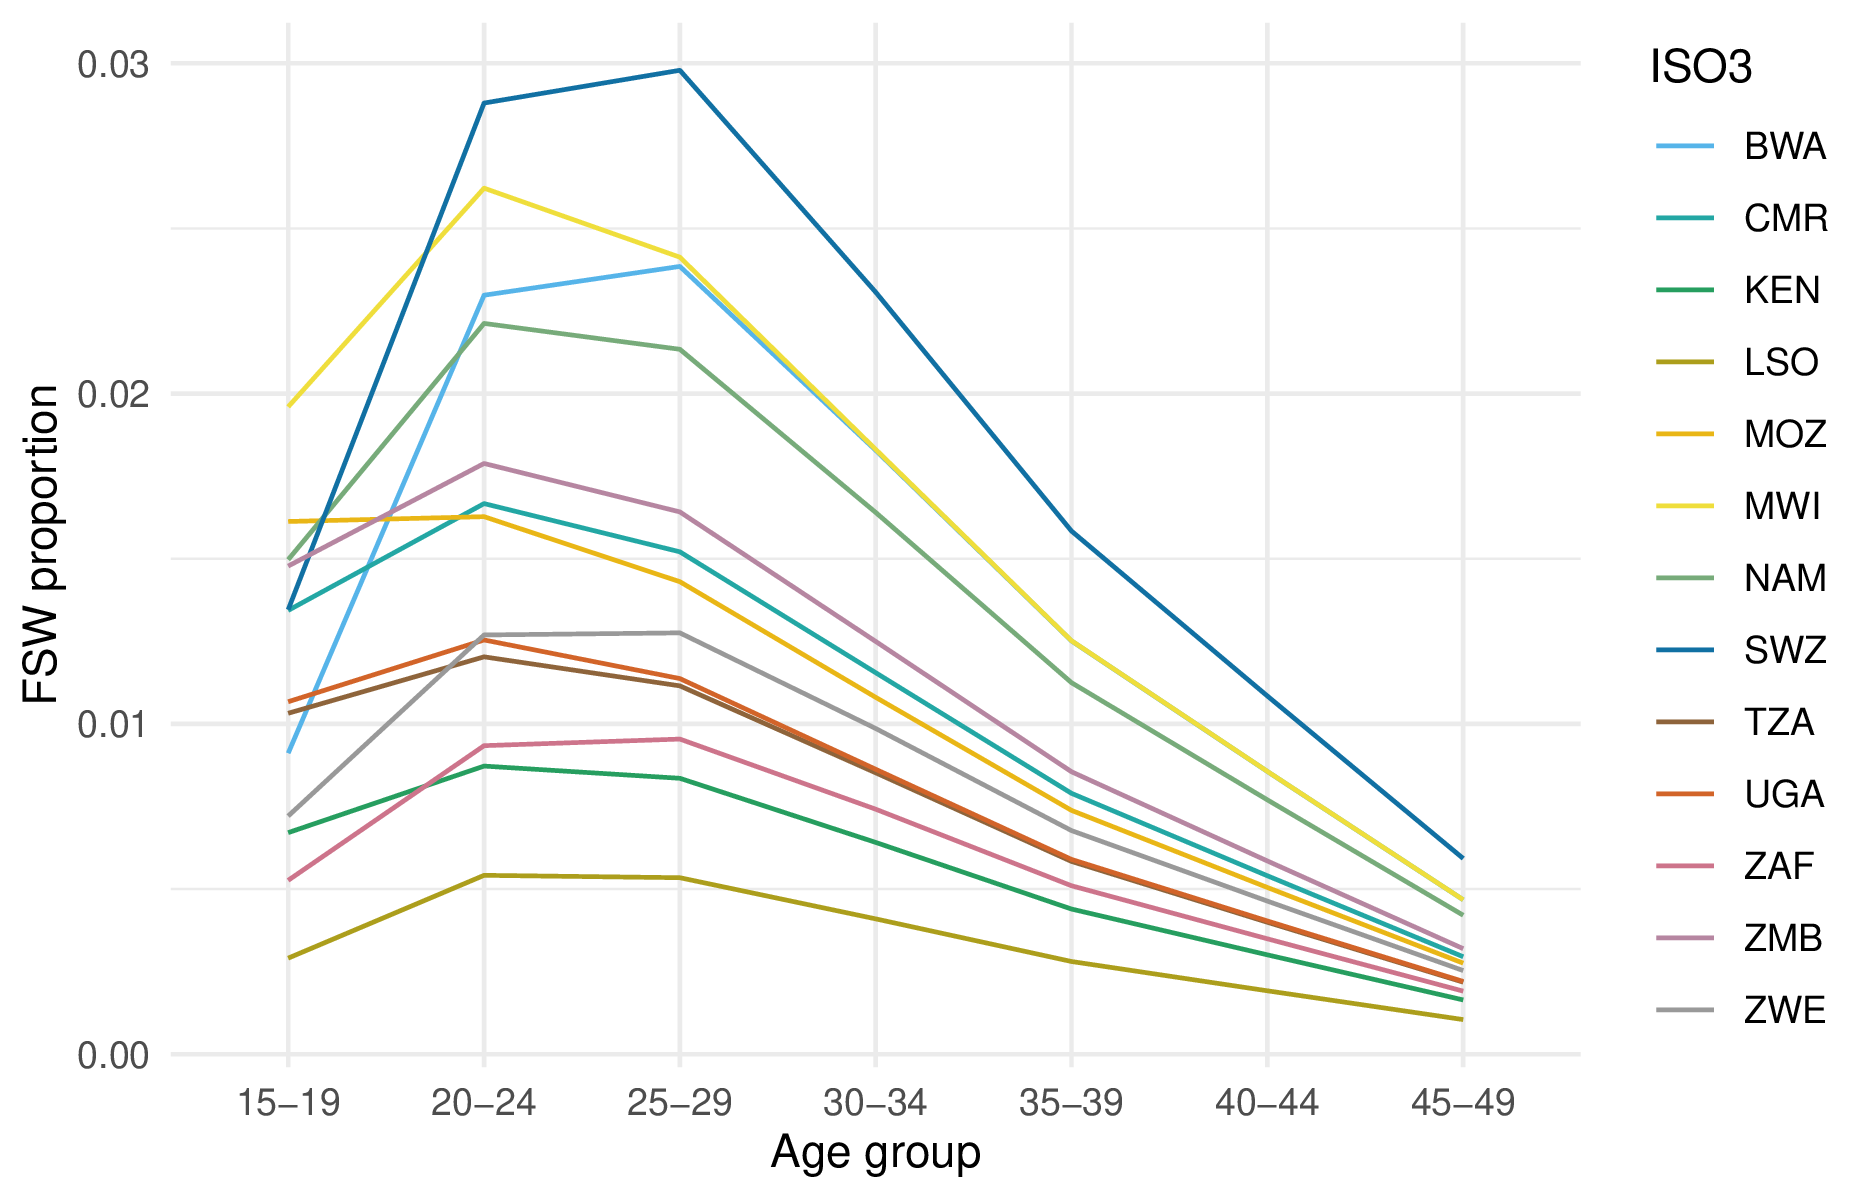
\includegraphics[width=0.9\linewidth]{figures/multi-agyw/age-disagg-fsw-line} 

}

\caption{Proportion of FSW by age group (including the age groups 30-34, 35-39, 40-44 and 45-49) as produced by the disaggregation procedure.}\label{fig:age-disagg-fsw-line}
\end{figure}

\hypertarget{results-2}{%
\subsection{Results}\label{results-2}}

\hypertarget{coverage-assessment-1}{%
\subsubsection{Coverage assessment}\label{coverage-assessment-1}}

\hypertarget{variance-decomposition}{%
\subsubsection{Variance decomposition}\label{variance-decomposition}}

\hypertarget{estimates}{%
\subsubsection{Estimates}\label{estimates}}

\hypertarget{prevalence-and-incidence-by-risk-group}{%
\section{Prevalence and incidence by risk group}\label{prevalence-and-incidence-by-risk-group}}

\hypertarget{disaggregation-of-naomi-estimates}{%
\subsection{Disaggregation of Naomi estimates}\label{disaggregation-of-naomi-estimates}}

I calculated HIV incidence \(\lambda_{iak}\) and number of new HIV infections \(I_{iak}\) stratified according to district, age group and risk group by linear disaggregation
\begin{align}
    I_{ia} &= \sum_k I_{iak} = \sum_k \lambda_{iak}N_{iak} \\
    &= 0 + \lambda_{ia2} N_{ia2} + \lambda_{ia3} N_{ia3} + \lambda_{ia4} N_{ia4} \\
    &= \lambda_{ia2} \left(N_{ia2}  + \text{RR}_{3} N_{ia3} + \text{RR}_4(\lambda_{ia}) N_{ia4}  \right).
\end{align}
Risk group specific HIV incidence estimates are then given by
\begin{align}
    \lambda_{ia1} &= 0, \\
    \lambda_{ia2} &= I_{ia} / \left(N_{ia2} + \text{RR}_{3} N_{ia3} + \text{RR}_4(\lambda_{ia}) N_{ia4}\right), \\
    \lambda_{ia3} &= \text{RR}_{3} \lambda_{ia2}, \\
    \lambda_{ia4} &= \text{RR}_4(\lambda_{ia}) \lambda_{ia2}.
\end{align}
which we evaluated using Naomi model estimates of the number of new HIV infections \(I_{ia} = \lambda_{ia} N_{ia}\), HIV infection risk ratios \(\{\text{RR}_3, \text{RR}_4(\lambda_{ia})\}\), and risk group population sizes as above.
The risk ratio \(\text{RR}_4(\lambda_{ia})\) was defined as a function of general population incidence.
The number of new HIV infections are then \(I_{iak} = \lambda_{iak} N_{iak}\).

\hypertarget{expected-new-infections-reached}{%
\subsection{Expected new infections reached}\label{expected-new-infections-reached}}

I calculated the number of new infections that would be reached prioritising according to each possible stratification of the population--that is for all \(2^3 = 8\) possible combinations of stratification by location, age, and risk group.
As an illustration, for stratification just by age, we aggregated the number of new HIV infections and HIV incidence as such
\begin{align}
    I_a &= \sum_{ik} I_{iak}, \\
    \lambda_a &= I_a / \sum_{ik} N_{iak}.
\end{align}
Under this stratification, individuals in each age group \(a\) are prioritised according to the highest HIV incidence \(\lambda_a\).
By cumulatively summing the expected infections, for each fraction of the total population reached we calculated the fraction of total expected new infections that would be reached.

This analysis was relatively simple.
More involved analyses might consider prioritisation of a hypothetical intervention which has some, possibly varying, probability of preventing HIV acquisition, as well as the costs associated to its roll-out.

\hypertarget{discussion-1}{%
\section{Discussion}\label{discussion-1}}

\hypertarget{distribution-of-risk}{%
\subsubsection{Distribution of risk}\label{distribution-of-risk}}

\begin{itemize}
\tightlist
\item
  Connection to phylogenetic results from BDI
\item
  About transmission rather than incidence
\item
  Only age-sex structured not age-sex-behaviour
\item
  Does not undermine my work
\end{itemize}

\hypertarget{community-engagement}{%
\subsubsection{Community engagement}\label{community-engagement}}

\begin{itemize}
\tightlist
\item
  CSO engagement
\item
  Problem in Malawi with FSW
\end{itemize}

\hypertarget{limitations-1}{%
\subsection{Limitations}\label{limitations-1}}

\hypertarget{conclusion-1}{%
\subsection{Conclusion}\label{conclusion-1}}

\hypertarget{naomi-aghq}{%
\chapter{Fast approximate deterministic Bayesian inference}\label{naomi-aghq}}

\adjustmtc
\markboth{Fast, approximate inference for the Naomi model}{}

Code for the analysis in this chapter is available from \href{https://github.com/athowes/elgm-inf}{\texttt{athowes/naomi-aghq}} and supported by the R package \href{https://athowes.github.io/inf.utils}{\texttt{inf.utils}}.
Include an edited version of the corresponding paper here.

\hypertarget{background-3}{%
\section{Background}\label{background-3}}

\hypertarget{the-naomi-model}{%
\section{The Naomi model}\label{the-naomi-model}}

\hypertarget{adaptive-gauss-hermite-quadrature}{%
\section{Adaptive Gauss-Hermite quadrature}\label{adaptive-gauss-hermite-quadrature}}

\hypertarget{malawi-case-study}{%
\section{Malawi case-study}\label{malawi-case-study}}

\hypertarget{discussion-2}{%
\section{Discussion}\label{discussion-2}}

\hypertarget{conclusions}{%
\chapter{Future work and conclusions}\label{conclusions}}

\adjustmtc
\markboth{Conclusions}{}

\hypertarget{future-work}{%
\section{Future work}\label{future-work}}

Avenues for future work include:

\begin{enumerate}
\def\labelenumi{\arabic{enumi}.}
\tightlist
\item
  Extending the risk group model described in Chapter \ref{multi-agyw} to include all adults 15-49. This may involve modelling of age-stratified sexual partnerships \autocite{wolock2021evaluating}. Such a model would likely fall out of the scope of \texttt{R-INLA}, but may be possible using \texttt{aghq} with Laplace marginals as described in Chapter \ref{naomi-aghq}.
\item
  Evaluating the accuracy of \texttt{aghq} with Laplace marginals for a greater variety of extended latent Gaussian models.
\end{enumerate}

\hypertarget{conclusions-1}{%
\section{Conclusions}\label{conclusions-1}}

The spatial structure chapter is interesting because:

\begin{itemize}
\tightlist
\item
  I designed experiments to thoroughly compare models for spatial structure using tools for model assessment such as proper scoring rules and posterior predictive checks.
\end{itemize}

The risk group chapter is interesting because:

\begin{itemize}
\tightlist
\item
  I estimated HIV risk group proportions for AGYW, enabling countries to prioritise their delivery of HIV prevention services.
\item
  I analysed the number of new infections that might be reached under a variety of risk stratification strategies.
\item
  I used \texttt{R-INLA} to specify multinomial spatio-temporal models via the Poisson-multinomial transformation. This includes complex two- and three-way Kronecker product interactions defined using the \texttt{group} and \texttt{replicate} options.
\end{itemize}

The fast, approximate inference chapter is interesting because:

\begin{itemize}
\tightlist
\item
  I developed a novel Bayesian inference method, motivated by a challenging and practically important problem in HIV inference.
\item
  The method enables integrated nested Laplace approximations to be fit to and studied on a wider class of models than was previously possible.
\item
  My implementation of the method was straightforward, building on the \texttt{TMB} and \texttt{aghq} packages, and described completely and accessibly in \textcite{howes2023fast}.
\end{itemize}

My final conclusions are:

\begin{itemize}
\tightlist
\item
  Modelling complex data, more often than not, pushes the boundaries of the statistical toolkit available
\item
  A challenge I encountered was the difficulty of implementing identical models across multiple frameworks with the aim of studying the inference method. Or, of a similarly fraught nature, comparing different models implemented in different frameworks with the aim of studying model differences. The frequently asked questions section of the \texttt{R-INLA} website \autocite{rinla2023faq} notes that, ``the devil is in the details''. I have resolved this challenge by using a given \texttt{TMB} model template to fit models using multiple inference methodologies: empirical Bayes with Gaussian marginals \autocite{kristensen2016tmb}, AGHQ with Gaussian marginals \autocite{stringer2021implementing}, AGHQ with Laplace marginals \autocite{howes2023fast}, and HMC using NUTS \autocite{monnahan2018no}. The benefits of such a ecosystem of packages are noted by \textcite{stringer2021fields}. I would particularly highlight the benefit of enabling analysts to easily vary their choice of inference method based on the stage of model development that they are in.
\item
  I have aimed to write this thesis, and the work described within it, in keeping with the principles of open science. I hope that doing so allows my work to be scrutinised, and, optimistically, built upon. This would not have been possible without a range of tools from the R ecosystem such as \texttt{rmarkdown} and \texttt{rticles}, as well as those developed within the MRC Centre for Global Infectious Disease Analysis like \texttt{orderly} and \texttt{didehpc}.
\end{itemize}

\startappendices

\hypertarget{the-first-appendix}{%
\chapter{The First Appendix}\label{the-first-appendix}}


%%%%% REFERENCES

% JEM: Quote for the top of references (just like a chapter quote if you're using them).  Comment to skip.
% \begin{savequote}[8cm]
% The first kind of intellectual and artistic personality belongs to the hedgehogs, the second to the foxes \dots
%   \qauthor{--- Sir Isaiah Berlin \cite{berlin_hedgehog_2013}}
% \end{savequote}

\setlength{\baselineskip}{0pt} % JEM: Single-space References

{\renewcommand*\MakeUppercase[1]{#1}%
\printbibliography[heading=bibintoc,title={\bibtitle}]}


\end{document}
